\documentclass[12pt,aspectratio=169]{beamer}

% ====================================================
% ====================================================
% USEPACKAGES AND IMPORTS
% ====================================================
% ====================================================

\usepackage[T1]{fontenc}
\usepackage[utf8]{inputenc}
\usepackage[english]{babel}

% tables
\usepackage{tabularx}
\usepackage{colortbl}
\usepackage{multirow}
\usepackage{makecell}

% tikz and colors
\usepackage{tikz}
\usepackage{xcolor}
\usepackage{pgfplots}
\usepackage{pgfplotstable}
\usepackage{tikzsymbols}

\usetikzlibrary{calc}
\usetikzlibrary{trees}
\usetikzlibrary{patterns}
\usetikzlibrary{shadings}
\usetikzlibrary{positioning}
\usetikzlibrary{intersections}
\usepgfplotslibrary{patchplots}
\usepgfplotslibrary{fillbetween}
\usetikzlibrary{decorations.pathreplacing}

\usetikzlibrary{arrows}
\usetikzlibrary{arrows.meta}

\usetikzlibrary{shapes}
\usetikzlibrary{shapes.arrows}
\usetikzlibrary{shapes.callouts}
\usetikzlibrary{shapes.symbols}
\usetikzlibrary{shapes.geometric}

% boxes
\usepackage[many]{tcolorbox}

% math packages and fonts
\usepackage{bm}
\usepackage{ccfonts}
\usepackage{eulervm}
\usepackage{amsmath}
\usepackage{amsfonts}
\usepackage{amssymb}
\usepackage{amsthm}
\usepackage{mathtools}
\usepackage{nicefrac}
\usepackage{slashed}
\usepackage{bbold}
\usepackage{array}
\usepackage{cancel}

% algorithms and listings
\usepackage[ruled,vlined,linesnumbered]{algorithm2e}
\usepackage{listings}
\usepackage{setspace}

\tcbuselibrary{listings}
\tcbuselibrary{breakable}
\tcbuselibrary{skins}

% misc
\usepackage{soul}
\usepackage{pifont}
\usepackage{skull}
\usepackage{multicol}
\usepackage{animate}
\usepackage{hyperref}
\usepackage{wasysym}
\usepackage[absolute,overlay]{textpos}
\usepackage[hang,flushmargin]{footmisc}

% ====================================================
% ====================================================
% LAYOUT AND THEME
% ====================================================
% ====================================================

\usetheme{Copenhagen}

% color definitions
\definecolor{myblue1}{RGB}{35,119,189}
\definecolor{myblue2}{RGB}{95,179,238}
\definecolor{myblue3}{RGB}{129,168,207}
\definecolor{myblue4}{RGB}{26,89,142}

\definecolor{myred1}{RGB}{247,12,12}

% set theme colors
\setbeamercolor*{structure}{fg=myblue1,bg=blue}
\setbeamercolor*{palette primary}{use=structure,fg=white,bg=structure.fg}
\setbeamercolor*{palette secondary}{use=structure,fg=white,bg=structure.fg!75!black}
\setbeamercolor*{palette tertiary}{use=structure,fg=white,bg=structure.fg!50!black}
\setbeamercolor*{palette quaternary}{fg=black,bg=white}

\setbeamertemplate{itemize item}[circle]
\setbeamertemplate{itemize subitem}[circle]
\setbeamertemplate{itemize subsubitem}[circle]

\setbeamertemplate{enumerate item}[circle]
\setbeamertemplate{enumerate subitem}[circle]
\setbeamertemplate{enumerate subsubitem}[circle]

\setbeamercolor{itemize item}{fg=myblue1}
\setbeamercolor{itemize subitem}{fg=myblue1}
\setbeamercolor{itemize subsubitem}{fg=myblue1}

\setbeamertemplate{section in toc}[circle]
\setbeamertemplate{subsection in toc}[circle]
\setbeamerfont{subsection in toc}{size=\scriptsize}

\setbeamercolor{frametitle continuation}{fg=black}

% title graphic -- sap logo and dhbw logo
\titlegraphic{
\includegraphics[scale=0.1]{../03_img/logo_sap}\hspace*{4.75cm}~%
   	
\includegraphics[scale=0.05]{../03_img/logo_dhbw}
}

\makeatletter
% frame title
\defbeamertemplate*{frametitle}{mydefault}[1][left]
{
  	\ifbeamercolorempty[bg]{frametitle}{}{\nointerlineskip}%
  	\nointerlineskip%
 	\@tempdima=\textwidth%
  	\advance\@tempdima by\beamer@leftmargin%
  	\advance\@tempdima by\beamer@rightmargin%
  	\begin{tcolorbox}[
  		enhanced,
  		outer arc=0pt,
  		arc=0pt,
  		boxrule=0pt,
  		top=0pt,
  		bottom=0pt,
  		enlarge left by=-\beamer@leftmargin,
  		enlarge right by=-\beamer@rightmargin,
  		width=\paperwidth,
  		nobeforeafter,
  		interior style={
    			left color=myblue2,
    			right color=white
    		},
  		shadow={0mm}{-0.4mm}{0mm}{black!60,opacity=0.6},    
  		shadow={0mm}{-0.8mm}{0mm}{black!40,opacity=0.4},    
  	]
    	\usebeamerfont{frametitle}%
    	\vbox{}\vskip-1ex%
    	\if@tempswa\else\csname beamer@fte#1\endcsname\fi%
    	\insertframetitle\par%
    	{%
      		\ifx\insertframesubtitle\@empty%
      		\else%
      		{\usebeamerfont{framesubtitle}\usebeamercolor[fg]{black}\insertframesubtitle\strut\par}%
      		\fi
    	}%
    	\vskip-1ex%
    	\if@tempswa\else\vskip-.3cm\fi
  	\end{tcolorbox}%
}

% footline of a frame
\defbeamertemplate*{footline}{mysplit theme}
{%
  	\leavevmode%
  	\hbox{
		\begin{beamercolorbox}[
			wd=.5\paperwidth,ht=2.5ex,dp=1.125ex,leftskip=.3cm plus1fill,rightskip=.3cm
		]{author in head/foot}%
    			\usebeamerfont{author in head/foot}\insertshortauthor\ (\insertinstitute), \insertdate
  		\end{beamercolorbox}%
  		\begin{beamercolorbox}[
			wd=.5\paperwidth,ht=2.5ex,dp=1.125ex,leftskip=.3cm,rightskip=.3cm plus1fil
		]{title in head/foot}%
    			\usebeamerfont{title in head/foot}\insertshorttitle\hfill
    			\insertprefix-\insertframenumber/\inserttotalframenumber\hspace*{0.5em}
  		\end{beamercolorbox}}%
  	\vskip0pt%
}
\makeatother

% ====================================================
% ====================================================
% COMMANDS AND GENERAL DEFINITIONS
% ====================================================
% ====================================================

% page number prefix
\newcommand\insertprefix{}  % empty by default
\newcommand\prefix[1]{\renewcommand\insertprefix{#1}}

% math definitions
% ====================================================
\DeclareMathOperator*{\argmax}{arg\,max}
\DeclareMathOperator*{\argmin}{arg\,min}
\newcommand*\diff{\mathop{}\!\mathrm{d}}

\newcommand*{\vertbar}{\rule[-1ex]{0.5pt}{2.5ex}}
\newcommand*{\horzbar}{\rule[.5ex]{2.5ex}{0.5pt}}

% commands
% ====================================================

% highlight commands
% --------------------------------------------------------------------------------------------------------
% highlight command
\newcommand{\highlight}[1]{\textcolor{myblue1}{\textbf{#1}}}
\newcommand{\highlighttt}[1]{\textcolor{myblue1}{\texttt{#1}}}
\newcommand{\Highlight}[1]{\textcolor{myred1}{\textbf{#1}}}

% blue color boxes (with frame/without frame/without fill)
\newtcolorbox{boxBlue}{colback=myblue1!10!white,colframe=myblue4}
\newtcolorbox{boxBlueNoFrame}{colback=myblue1!10!white,colframe=myblue1!10!white}
\newtcolorbox{boxBlueNoFill}{colback=white,colframe=myblue4}

% font commands
% --------------------------------------------------------------------------------------------------------
\newcommand{\linkstyle}[1]{\underline{\smash{\texttt{#1}}}} 		% style of hyperlinks

% tikz commands
% --------------------------------------------------------------------------------------------------------

% yellow sticky note
\newcommand{\bubble}[3]{
\begin{textblock}{100}(#1, #2)
      	\begin{tikzpicture}
		\node[rectangle,draw=yellow,very thick,fill=yellow!60,align=center] at (0,0) {#3};
	\end{tikzpicture}
\end{textblock}
}

\newcommand{\floattext}[3]{
\begin{textblock}{100}(#1, #2)
      	#3
\end{textblock}
}

\newcommand{\doublecircle}[2]{
	\draw[fill=white,draw=myblue1] (#1,#2) circle (2mm);
	\draw[fill=myblue1,draw=myblue1] (#1,#2) circle (1.5mm);
}

% slide modifiers
% --------------------------------------------------------------------------------------------------------
% mark slide as optional
\newcommand{\optional}{
	\begin{textblock}{100}(0.15,0.30)
      		
\includegraphics[scale=0.2]{../03_img/scream}
    	\end{textblock}
}

% mark slide as important
\newcommand{\important}{
	\begin{textblock}{100}(0.10,0.15)
      		
\includegraphics[scale=0.1]{../03_img/important}
    	\end{textblock}
}

% citation
% --------------------------------------------------------------------------------------------------------
% first argument in {book, online, article}
\newcommand{\literature}[5]{
	\setbeamertemplate{bibliography item}[#1]
	\bibitem{#2}
	\highlight{#3} \\
	\textcolor{darkgray}{\textit{#4}} \\
	\textcolor{black}{#5}
}
% cite content
\newcommand{\citeAuthor}[3]{\vfill\scriptsize\textcolor{lightgray}{#1 \cite{#2} #3}}

% slide architecture
% --------------------------------------------------------------------------------------------------------
% divide frame into two parts
\newcommand{\divideTwo}[4]{
	\begin{minipage}{#1\textwidth}
		#2
	\end{minipage}
	\hfill
	\begin{minipage}{#3\textwidth}
		#4
	\end{minipage}
}

% divide frame into two parts (start on top)
\newcommand{\divideTwoTop}[4]{
	\begin{minipage}[t]{#1\textwidth}
		#2
	\end{minipage}
	\hfill
	\begin{minipage}[t]{#3\textwidth}
		#4
	\end{minipage}
}

% special pages
% --------------------------------------------------------------------------------------------------------
% title page
\newcommand{\maketitlepage}{
	{
		\beamertemplatenavigationsymbolsempty
		\usebackgroundtemplate{%
			\tikz[overlay,remember picture] \node[opacity=0.2, at=(current page.center)] {
  				
\includegraphics[height=\paperheight,width=\paperwidth]{../03_img/processor.jpg}
			};
		}
		\begin{frame}[plain]
			\vspace*{0.75cm}
			\maketitle
			\vfill
			\begin{center}
				\footnotesize Find all slides on \href{https://github.com/DaWe1992/Applied_ML_Fundamentals}{\linkstyle{GitHub}}
			\end{center}
		\end{frame}
	}
}

% divider page
\newcommand{\makedivider}[1]{
	{
		\beamertemplatenavigationsymbolsempty
		\usebackgroundtemplate{%
			\tikz[overlay,remember picture] \node[opacity=0.2, at=(current page.center)] {
  				
\includegraphics[height=\paperheight,width=\paperwidth]{../03_img/processor.jpg}
			};
		}
		\begin{frame}[plain]
			\vfill
			\begin{boxBlue}
				\centering
				\textbf{Section:} \\
				\large \highlight{#1}
			\end{boxBlue}
			\vfill
			\centering
			
\includegraphics[scale=0.05]{../03_img/logo_dhbw.png}
			\vfill
		\end{frame}
	}
}

% overview page
\newcommand{\makeoverview}[1]{
	\begin{frame}{Lecture Overview}{}
		\begin{tabbing}
			\hspace*{3.5cm}\= \kill
			\ifnum #1=1 \highlight{\textbf{Unit I:}} \else \textbf{Unit I:} \fi
			\> \ifnum #1=1 \highlight{Machine Learning Introduction} \else Machine Learning Introduction \fi \\
		\end{tabbing}
	\end{frame}
}

% thank you page
\newcommand{\makethanks}{
	{\beamertemplatenavigationsymbolsempty
	\begin{frame}[plain]
		\vfill
		\begin{boxBlue}
			\centering
			\Large \highlight{Thank you very much for the attention!}
		\end{boxBlue}
		
		\vfill\footnotesize
		\begin{tabbing}
			\hspace*{1.5cm}\= \kill
			\highlight{Topic:} 	\> \inserttitle \\
			\highlight{Date:} 	\> \insertdate
		\end{tabbing}
		
		\vfill
		\highlight{Contact:} \\
		\insertauthor\ (D062271) \\
		\insertinstitute \\
		\href{mailto:daniel.wehner@sap.com}{\linkstyle{daniel.wehner@sap.com}}
		
		\vfill\normalsize
		\begin{center}
			\large\highlight{Do you have any questions?}
		\end{center}
		\vfill
	\end{frame}}
}

% global pfgplots settings
% --------------------------------------------------------------------------------------------------------
\pgfplotsset{
	% allow filtering of data for pgfplots
	discard if/.style 2 args={
        		x filter/.code={
            		\edef\tempa{\thisrow{#1}}
            		\edef\tempb{#2}
            		\ifx\tempa\tempb
                		\def\pgfmathresult{inf}
            		\fi
        		}
    	},
    	discard if not/.style 2 args={
        		x filter/.code={
            		\edef\tempa{\thisrow{#1}}
            		\edef\tempb{#2}
            		\ifx\tempa\tempb
            		\else
                		\def\pgfmathresult{inf}
            		\fi
        		}
    	}
}


% ====================================================
% ====================================================
% PRESENTATION DATA
% ====================================================
% ====================================================

\title[Classification I]{*** Applied Machine Learning Fundamentals *** Decision Trees and Ensembles}
\institute{SAP\,SE}
\author{Daniel Wehner}
\date{\today}
\prefix{DT}

% ====================================================
% ====================================================
% BEGIN OF DOCUMENT
% ====================================================
% ====================================================

\begin{document}

% Title frame
%______________________________________________________________________
\maketitlepage


% Agenda
%______________________________________________________________________
\begin{frame}{Agenda \today}
	\begin{multicols}{2}
		\tableofcontents
	\end{multicols}
\end{frame}


% Section: Introduction
%______________________________________________________________________
\section{Introduction}
\makedivider{Introduction}

% What we want...
\begin{frame}{What we want...}{}
	\divideTwo{0.49}{
		\vspace*{4mm}
		\begin{table}
	\scalebox{0.6}{
	\begin{tabular}{| c | c | c | c || c |}
		\hline
		\highlight{Outlook} 		&
		\highlight{Temperature} 	&
		\highlight{Humidity} 		&
		\highlight{Wind} 			&
		\highlight{PlayGolf}		\\ \hline\hline
		sunny 	& hot 			& high 		& weak 		& \textbf{no}		\\ \hline
		sunny 	& hot 			& high 		& strong 	& \textbf{no} 		\\ \hline
		overcast 	& hot 			& high 		& weak 		& \textbf{yes} 		\\ \hline
		rainy 	& mild 			& high 		& weak 		& \textbf{yes} 		\\ \hline
		rainy 	& cool 			& normal 	& weak 		& \textbf{yes} 		\\ \hline
		rainy 	& cool 			& normal 	& strong 	& \textbf{no} 		\\ \hline
		overcast 	& cool 			& normal 	& strong 	& \textbf{yes} 		\\ \hline
		sunny 	& mild 			& high 		& weak 		& \textbf{no} 		\\ \hline
		sunny 	& cool 			& normal 	& weak 		& \textbf{yes} 		\\ \hline
		rainy 	& mild 			& normal 	& weak 		& \textbf{yes}		\\ \hline
		sunny 	& mild 			& normal 	& strong 	& \textbf{yes} 		\\ \hline
		overcast 	& mild 			& high 		& strong 	& \textbf{yes} 		\\ \hline
		overcast 	& hot 			& normal 	& weak 		& \textbf{yes}		\\ \hline
		rainy 	& mild 			& high 		& strong 	& \textbf{no} 		\\ \hline\hline
		rainy 	& mild 			& normal	& strong		& \highlight{???}		\\ \hline
	\end{tabular}}
\end{table}
	}{0.49}{
		% Set the overall layout of the tree
\tikzstyle{level 1}=[level distance=2.5cm, sibling distance=2cm]
\tikzstyle{level 2}=[level distance=2.5cm, sibling distance=2cm]

% Define styles for bags and leafs
\tikzstyle{bag}=[rectangle,draw=black,text width=4em,text centered]
\tikzstyle{end}=[circle,draw=black,minimum width=3pt,fill,inner sep=0pt]

\begin{figure}
	\centering
	\begin{tikzpicture}[
		scale=0.9,
		every node/.style={scale=0.9},
		sloped
	]
		\node[bag]{\highlight{Outlook}}
    		child{
        		node[bag]{\highlight{Humid.}}        
        		child {
            	    		node[end,label=below:{\textbf{\underline{No}}}]{}
            	    		edge from parent
            		    	node[above]{\textit{high}}
            		}
            		child{
                		node[end,label=below:{\textbf{\underline{Yes}}}]{}
                		edge from parent
                		node[above]{\textit{normal}}
            		}
        		edge from parent         
            		node[above]{\textit{sunny}}
		}
		child{
			node[end,label=below:{\textbf{\underline{Yes}}}]{}
			edge from parent
			node[above]{\textit{overcast}}
		}
		child{
        		node[bag]{\highlight{Wind}}        
            		child{
                		node[end,label=below:{\textbf{\underline{No}}}]{}
                		edge from parent
                		node[above]{\textit{strong}}
            		}
            		child{
                		node[end,label=below:{\textbf{\underline{Yes}}}]{}
               		edge from parent
                		node[above]{\textit{weak}}
            		}
            		edge from parent 
            		node[above]{\textit{rainy}}
    		};
	\end{tikzpicture}
\end{figure}
	}
\end{frame}


% What are Decision Trees?
\begin{frame}{What are Decision Trees?}{}
	\begin{itemize}
		\item Decision trees are induced in a \highlight{supervised} fashion
		\item Originally invented by \textit{Ross Quinlan} (1986)
		\item Decision trees are grown \textbf{recursively} $\rightarrow$ \textit{'divide-and-conquer'}
		\item A decision tree consists of:

		\begin{tabbing}
			\hspace*{2.5cm}\= \kill
			\textbf{Nodes}	\>	Each node corresponds to an attribute test 	\\
			\textbf{Edges}	\>	One edge per possible test outcome			\\
			\textbf{Leaves}	\>	Class label to predict
		\end{tabbing}
	\end{itemize}
\end{frame}


% Classifying new Instances
\begin{frame}{Classifying new Instances}{}
	\divideTwo{0.49}{
		\begin{itemize}
			\item Suppose we get a new instance:
			
			\footnotesize
			\begin{tabbing}
				\hspace*{2.5cm}\= \kill
				\texttt{Outlook}			\>	rainy		\\
				\texttt{Temperature} 		\>	mild	 	\\
				\texttt{Humidity}			\>	normal	\\
				\texttt{Wind}			\>	strong
			\end{tabbing}
			\normalsize

			\item \textbf{What is its class?}
			\item Answer: \textbf{No}
		\end{itemize}
	}{0.49}{
		% Set the overall layout of the tree
\tikzstyle{level 1}=[level distance=2.5cm, sibling distance=2cm]
\tikzstyle{level 2}=[level distance=2.5cm, sibling distance=2cm]

% Define styles for bags and leafs
\tikzstyle{bag}=[rectangle,draw=black,text width=4em,text centered]
\tikzstyle{end}=[circle,draw=black,minimum width=3pt,fill,inner sep=0pt]

\begin{figure}
	\centering
	\begin{tikzpicture}[
		scale=0.9,
		every node/.style={scale=0.9},
		sloped
	]
		\node[bag]{\highlight{Outlook}}
    		child{
        		node[bag]{\highlight{Humid.}}        
        		child {
            	    		node[end,label=below:{\textbf{\underline{No}}}]{}
            	    		edge from parent
            		    	node[above]{\textit{high}}
            		}
            		child{
                		node[end,label=below:{\textbf{\underline{Yes}}}]{}
                		edge from parent
                		node[above]{\textit{normal}}
            		}
        		edge from parent         
            		node[above]{\textit{sunny}}
		}
		child{
			node[end,label=below:{\textbf{\underline{Yes}}}]{}
			edge from parent
			node[above]{\textit{overcast}}
		}
		child{
        		node[bag]{\highlight{Wind}}        
            		child{
                		node[end,label=below:{\textbf{\underline{No}}}]{}
                		edge from parent
                		node[above]{\textit{strong}}
            		}
            		child{
                		node[end,label=below:{\textbf{\underline{Yes}}}]{}
               		edge from parent
                		node[above]{\textit{weak}}
            		}
            		edge from parent 
            		node[above]{\textit{rainy}}
    		};
	\end{tikzpicture}
\end{figure}
	}
\end{frame}


% Another Decision Tree...
\begin{frame}{Another Decision Tree...}{}
	\bubble{1}{11}{\footnotesize \textbf{Is this one better?}}
	\vspace*{-2mm}
	{
% Set the overall layout of the tree
\tikzstyle{level 1}=[level distance=2cm,sibling distance=6cm]
\tikzstyle{level 2}=[level distance=2.5cm,sibling distance=2cm]
\tikzstyle{level 3}=[level distance=2.5cm,sibling distance=1.5cm]

% Define styles for bags and leafs
\tikzstyle{bag}=[rectangle,draw=black,text width=4em,text centered]
\tikzstyle{end}=[circle,draw=black,minimum width=3pt,fill,inner sep=0pt]

\begin{figure}
	\centering
	\begin{tikzpicture}[
		scale=0.55,
		every node/.style={scale=0.5},
		sloped
	]
		\node[bag]{\highlighttt{Temp.}}
    		child {
     	   		node[bag]{\highlighttt{Outlook}}        
            		child {
                			node[end, label=below:{\textbf{\underline{No}}}]{}
                			edge from parent
                			node[above]{\textit{sunny}}
            		}
            		child {
                			node[end, label=below:{\textbf{\textcolor{red}{\underline{?}}}}]{}
               			edge from parent
                			node[above]{\textit{rain}}
            		}
			child {
                			node[end, label=below:{\textbf{\underline{Yes}}}]{}
               			edge from parent
                			node[above]{\textit{overcast}}
            		}
            		edge from parent 
            		node[above]{\textit{hot}}
    		}
		child {
        			node[bag]{\highlighttt{Outlook}}        
        			child {
                			node[bag]{\highlighttt{Humid.}}
                			child {
                				node[end, label=below:{\textbf{\underline{No}}}]{}
                				edge from parent
                				node[above]{\textit{high}}
                			}
				child {
                				node[end, label=below:{\textbf{\underline{Yes}}}]{}
                				edge from parent
                				node[above]{\textit{normal}}
                			}
				child[missing]{}
                			edge from parent
                			node[above]{\textit{sunny}}
            		}
            		child {
                			node[bag]{\highlighttt{Humid.}}
				child[missing]{}
				child {
					node[bag]{\highlighttt{Wind}}
					child {
						node[end, label=below:{\textbf{\underline{No}}}]{}
                					edge from parent
                					node[above]{\textit{strong}}
					}
					child {
						node[end, label=below:{\textbf{\underline{Yes}}}]{}
                					edge from parent
                					node[above]{\textit{weak}}
					}
					edge from parent
                				node[above]{\textit{high}}
				}
				child {
					node[end, label=below:{\textbf{\underline{Yes}}}]{}
                				edge from parent
                				node[above]{\textit{normal}}
				}
                			edge from parent
                			node[above]{\textit{rainy}}
            		}
			child {
                			node[end, label=below:{\textbf{\underline{Yes}}}]{}
                			edge from parent
                			node[above]{\textit{overcast}}
            		}
        			edge from parent         
            		node[above]{\textit{mild}}
		}
    		child {
        			node[bag]{\highlighttt{Outlook}}        
        			child {
                			node[end, label=below:{\textbf{\underline{Yes}}}]{}
                			edge from parent
                			node[above]{\textit{sunny}}
            		}
            		child {
                			node[bag]{\highlighttt{Humid.}}
                			child {
                				node[end, label=below:{\textbf{\textcolor{red}{\underline{?}}}}]{}
                				edge from parent
                				node[above]{\textit{high}}
                			}
				child {
                			node[bag]{\highlighttt{Wind}}
					child {
                					node[end, label=below:{\textbf{\underline{No}}}]{}
                					edge from parent
                					node[above]{\textit{strong}}
                				}
					child {
                					node[end, label=below:{\textbf{\underline{Yes}}}]{}
                					edge from parent
                					node[above]{\textit{weak}}
                				}
                				edge from parent
                				node[above]{\textit{normal}}
                			}
                			edge from parent
                			node[above]{\textit{rainy}}
            		}
			child {
                			node[end, label=below:{\textbf{\underline{Yes}}}]{}
                			edge from parent
                			node[above]{\textit{overcast}}
            		}
        			edge from parent         
            		node[above]{\textit{cool}}
		};
	\end{tikzpicture}
\end{figure}}
\end{frame}


% Inductive Bias of Decision Trees
\begin{frame}{Inductive Bias of Decision Trees}{}
	\divideTwo{0.75}{
		\begin{itemize}
			\item Complex models tend to \textbf{overfit} the data and do not generalize well
			\item Small decision trees are preferred
			\vspace*{4mm}
			\begin{boxBlueNoFrame}
				\textbf{Occam's razor}: \\
				\footnotesize \textbf{`More things should not be used than are necessary.'}
			\end{boxBlueNoFrame}
			\vspace*{2mm}
			\item \highlight{Prefer the simplest hypothesis that fits the data!}
		\end{itemize}
	}{0.20}{
		\begin{figure}
			\centering
			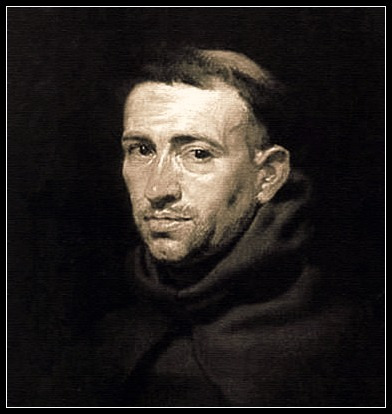
\includegraphics[scale=0.25]{08_decision_trees/02_img/william_of_ockham}
		\end{figure}
	}
\end{frame}


% The Root of all Evil... Which Attribute to choose?
\begin{frame}{The Root of all Evil... Which Attribute to choose?}{}
	\divideTwo{0.49}{
		% Set the overall layout of the tree
\tikzstyle{level 1}=[level distance=3.5cm, sibling distance=2cm]
\tikzstyle{level 2}=[level distance=3.5cm, sibling distance=2cm]

% Define styles for bags and leafs
\tikzstyle{bag} = [rectangle, draw=black, text width=4em, text centered]
\tikzstyle{end} = [circle, draw=black, minimum width=3pt, fill, inner sep=0pt]

\begin{figure}
	\centering
	\begin{tikzpicture}[
		scale=0.6,
		every node/.style={scale=0.5},
		sloped
	]
		\node[bag]{\highlight{Outlook}}
		child{
			node[bag,align=center]{Yes Yes\\No No\\No}
			edge from parent
			node[above]{\textit{sunny}}
		}
    		child{
			node[bag,align=center]{Yes Yes\\Yes Yes}
			edge from parent
			node[above]{\textit{overcast}}
		}
		child{
			node[bag,align=center]{Yes Yes\\Yes No\\No}
			edge from parent
			node[above]{\textit{rainy}}
		};
	\end{tikzpicture}
\end{figure}
		\vspace*{0.25mm}	
	}{0.49}{
		{
% Set the overall layout of the tree
\tikzstyle{level 1}=[level distance=3.5cm, sibling distance=2cm]
\tikzstyle{level 2}=[level distance=3.5cm, sibling distance=2cm]

% Define styles for bags and leafs
\tikzstyle{bag} = [rectangle, draw=black, text width=4em, text centered]
\tikzstyle{end} = [circle, draw=black, minimum width=3pt, fill, inner sep=0pt]

\begin{figure}
	\centering
	\begin{tikzpicture}[
		scale=0.6,
		every node/.style={scale=0.5},
		sloped
	]
		\node[bag]{\highlight{Temp.}}
		child {
			node[bag,align=center]{Yes Yes\\No No}
			edge from parent
			node[above]{\textit{hot}}
		}
    		child {
			node[bag,align=center]{Yes Yes\\Yes Yes\\No No}
			edge from parent
			node[above]{\textit{mild}}
		}
		child {
			node[bag,align=center]{Yes Yes\\Yes No}
			edge from parent
			node[above]{\textit{cool}}
		};
	\end{tikzpicture}
\end{figure}}
		\vspace*{0.25mm}	
	}

	\divideTwo{0.49}{
		{
% Set the overall layout of the tree
\tikzstyle{level 1}=[level distance=3.5cm, sibling distance=2cm]
\tikzstyle{level 2}=[level distance=3.5cm, sibling distance=2cm]

% Define styles for bags and leafs
\tikzstyle{bag} = [rectangle, draw=black, text width=4em, text centered]
\tikzstyle{end} = [circle, draw=black, minimum width=3pt, fill, inner sep=0pt]

\begin{figure}
	\centering
	\begin{tikzpicture}[
		scale=0.6,
		every node/.style={scale=0.5},
		sloped
	]
		\node[bag]{\highlight{Wind}}
		child {
			node[bag,align=center]{Yes Yes\\Yes Yes\\Yes Yes\\No No}
			edge from parent
			node[above]{\textit{strong}}
		}
		child {
			node[bag,align=center]{Yes Yes\\Yes No\\No No}
			edge from parent
			node[above]{\textit{weak}}
		};
	\end{tikzpicture}
\end{figure}}
	}{0.49}{
		{
% Set the overall layout of the tree
\tikzstyle{level 1}=[level distance=3.5cm, sibling distance=2cm]
\tikzstyle{level 2}=[level distance=3.5cm, sibling distance=2cm]

% Define styles for bags and leafs
\tikzstyle{bag} = [rectangle, draw=black, text width=4em, text centered]
\tikzstyle{end} = [circle, draw=black, minimum width=3pt, fill, inner sep=0pt]

\begin{figure}
	\centering
	\begin{tikzpicture}[
		scale=0.55,
		every node/.style={scale=0.5},
		sloped
	]
		\node[bag]{\highlighttt{Humid.}}
		child {
			node[bag,align=center]{Yes Yes\\Yes No\\No No\\No}
			edge from parent
			node[above]{\textit{high}}
		}
		child {
			node[bag,align=center]{Yes Yes\\Yes Yes\\Yes Yes\\No}
			edge from parent
			node[above]{\textit{normal}}
		};
	\end{tikzpicture}
\end{figure}}
	}
\end{frame}


% Finding a proper Attribute
\begin{frame}{Finding a proper Attribute}{}
	\divideTwo{0.79}{
		\begin{itemize}
			\item Simple and small trees are preferred
			\begin{itemize}
				\item Data in successor node should be \textbf{as pure as possible}
				\item I.\,e. nodes containing one class only are preferable
			\end{itemize}
			\item \textbf{Question:} How can we express this thought as a mathematical formula?
			\item \textbf{Answer:}
			\begin{itemize}
				\item \highlight{Entropy} (\textit{Claude E. Shannon})
				\item Originates in the field of \textbf{information theory}
			\end{itemize}
		\end{itemize}
	}{0.19}{
		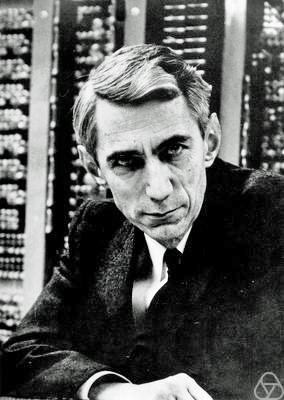
\includegraphics[scale=0.3]{08_decision_trees/02_img/claude_shannon}
	}
\end{frame}


% Measure of Impurity: Entropy
\begin{frame}{Measure of Impurity: Entropy}{}
	\begin{itemize}
		\item Entropy is a measure of chaos in the data (measured in bits)
		\item \textbf{Example:} Consider two classes $A$ and $B$ ($\mathcal{C} = \{ A, B \}$)
	
		\footnotesize
		\begin{tabbing}
			\hspace*{5cm}\=\hspace*{1.5cm}\= \kill
			$E(\{ \bm{A}, \bm{A}, \bm{A}, \bm{A}, \bm{A}, \bm{A}, \bm{A}, \bm{A} \})$
				\>	$\rightarrow$ 0		\>	$Bits$	\\
			$E(\{ \bm{A}, \bm{A}, \bm{A}, \bm{A}, \bm{A}, \bm{A}, B, B \})$
				\>	$\rightarrow$ 0.81 	\>	$Bits$	\\
			$E(\{ \bm{A}, \bm{A}, \bm{A}, \bm{A}, B, B, B, B \})$
				\>	$\rightarrow$ 1		\>	$Bit$		\\
			$E(\{ \bm{A}, \bm{A}, B, B, B, B, B, B \})$
				\>	$\rightarrow$ 0.81 	\>	$Bits$	\\
			$E(\{ B, B, B, B, B, B, B, B \})$	
				\>	$\rightarrow$ 0		\>	$Bits$
		\end{tabbing}
		\normalsize
	\end{itemize}
	
	\begin{boxBlueNoFrame}
		\footnotesize
		\highlight{If both classes are equally distributed, the entropy function $E$ reaches its maximum.
		Pure data sets have minimal entropy}.
	\end{boxBlueNoFrame}
\end{frame}


% Measure of Impurity: Entropy (Ctd.)
\begin{frame}{Measure of Impurity: Entropy (Ctd.)}{}
	\begin{figure}
	\centering
	\begin{tikzpicture}
    
    		\begin{axis}[
			scale=0.7,
			xlabel={Relative frequency of class $A$ ($p_A$)},
			ylabel={Entropy $E(\mathcal{D})$},
			grid=both,
    			grid style={line width=.1pt, draw=gray!10},
			minor tick num=2,
    			major grid style={line width=.2pt,draw=gray!80},
			minor grid style={line width=.2pt,draw=gray!30},
  			x=10cm,
  			y=5.5cm
		]

			\pgfplotstableread{08_decision_trees/05_data/data_entropy.txt} \datatable
			\addplot[myblue1,no marks,ultra thick,smooth] table[x=x,y=y] from \datatable;

			\node[fill=myblue1] at (axis cs:0.5,0.45) {\footnotesize $\textcolor{white}{E(\mathcal{D}) =
				-\sum_{c \in \mathcal{C}} p_c \cdot \log_2 p_c}$};
		
		\end{axis}
	\end{tikzpicture}
\end{figure}
\end{frame}


% Measure of Impurity: Entropy (Ctd.)
\begin{frame}{Measure of Impurity: Entropy (Ctd.)}{}
	\begin{boxBlueNoFrame}
		\highlight{Entropy formula:}
		\begin{equation}
			E(\mathcal{D}) = -\sum_{c \in \mathcal{C}} p_c \cdot \log_2 p_c
		\end{equation}
	\end{boxBlueNoFrame}

	\begin{itemize}
		\item Where $p_c$ denotes the relative frequency of class $c \in \mathcal{C}$	
		\item \textbf{Weather data:}
		\begin{align*}
			\mathcal{C} &= \{ yes, no \} \qquad \text{i.\,e.} \qquad
				p_{yes} = \nicefrac{9}{14} \quad \text{and} \quad p_{no} = \nicefrac{5}{14} \\[3mm]
			E(\mathcal{D})
				&= -\sum_{c \in \mathcal{C}} p_c \cdot \log_2 (p_c)
	       		   	= - (\nicefrac{9}{14} \cdot \log_2 (\nicefrac{9}{14}) + \nicefrac{5}{14} \cdot \log_2 (\nicefrac{5}{14}))
				= \boldsymbol{0.9403}
		\end{align*}
	\end{itemize}
\end{frame}


% Section: Wrap-Up
%______________________________________________________________________
\section{Wrap-Up}
\makedivider{Wrap-Up}

% Subsection: Summary
% --------------------------------------------------------------------------------------------------------
\subsection{Summary}

% Summary
\begin{frame}{Summary}{}

\end{frame}


% Subsection: Lecture Overview
% --------------------------------------------------------------------------------------------------------
\subsection{Lecture Overview}

\makeoverview{3}


% Subsection: Self-Test Questions
% --------------------------------------------------------------------------------------------------------
\subsection{Self-Test Questions}

% Self-Test Questions
\begin{frame}{Self-Test Questions}{}

\end{frame}


% Subsection: Recommended Literature and further Reading
% --------------------------------------------------------------------------------------------------------
\subsection{Recommended Literature and further Reading}

% Literature
%______________________________________________________________________
\begin{frame}{Recommended Literature and further Reading}{}
	\footnotesize
	\begin{thebibliography}{2}

	\end{thebibliography}
\end{frame}


% Thank you
%______________________________________________________________________
\makethanks

\end{document}